\documentclass{article}

\usepackage{graphicx}

\oddsidemargin 0.0in
\evensidemargin 0.0in
\textwidth 6.5in
\headheight 0.0in
\topmargin  0.0in
\textheight 9.0in

\title{SORTS Tech Report}
\author{Sam Wintermute, Joseph Xu, James Irizarry}

\begin{document}
\maketitle

\section{Overview}

The goal of this project is to interface Soar to a real-time strategy
(RTS) game. RTS games, such as StarCraft, WarCraft, and Command and
Conquer, are multi-player strategy games where a player needs to handle
many different tasks- planning base layouts, managing economies,
organizing attacks, responding to enemy attacks, and even diplomacy.
This is all occuring in real time (as the name implies), presenting an
extremely rich, challenging environment for an AI system. Making this
environment accessible to Soar provides many opportunities for both
utilizing existing capabilities and the development of new capabilities.

\subsection{ORTS Overview}

The Open Real Time Strategy software is a highly configurable game
engine used to play real time strategy (RTS) games \cite{ORTS}. The main
purpose for ORTS is to serve as an open source, open interface RTS game
engine for RTS AI tournaments. ORTS is undergoing active development as
of July 2006 at the University of Alberta under the direction of Michael
Buro.

There are several reasons why ORTS is especially suitable for use in
AI tournaments. It has a (relatively) straightforward C++ API, making
interfacing with your favorite AI system easy. All the specific game
mechanics, ranging from types of units, actions, and physics, are
specified via C++ style scripts called blueprints. This means that ORTS
can be easily configured to simulate a wide range of environments,
from arbitrarily simple ones like Wumpus World to complex ones like
Starcraft. Finally, ORTS has a client/server architecture in which
the server maintains the state of the world and only report to the
clients information they are supposed to have for a fair game. This
is in contrast to most commercial RTS games, in which each client
maintains the entire world state and prevents the player from accessing
forbidden information such as other players' locations only by hiding
them from the GUI. The result is that ORTS is impervious to "memory
hack" cheats that are widespread in commercial RTS games. This feature
is particularly important if tournaments are to be run across the
Internet.

\subsection{SORTS Overview}

SORTS is our middleware system that allows Soar to act as a client to
the ORTS game server, so that ORTS game playing agents can be written
in and executed on Soar. SORTS is much more than an interface bridge,
in that it provides fairly complex perception and action systems to the
Soar agent.

The low-level interface to ORTS is essentially a list of objects in the
world, each of which has a set of attributes (like x,y position, health,
owner, and size and shape information), and each of which can take any
of several low-level commands (such as "move", "shoot", or "build"). The
goal of our system is to build on this interface to give the Soar agent
a similar interface to a human playing the game. Some of this entails
adding fairly complex action controllers in the middleware, to replace
what a GUI would provide a human. A person playing a commercial RTS
such as StarCraft can command a unit to move to a location and build a
building in one click, and can send large groups to attack the enemy
semi-autonomously. Low-level behaviors like pathfinding and attack
micromanagement should not be things the Soar agent is concerned with-
the Soar agent should make decisions on the level of when and where to
build and when and where to attack, not how to avoid an obstacle in a
units path.

Similarly, the agent's perceptions need not be on a very low level.
Humans are rarely concerned with the exact x,y positions of the hundreds
of units in their control, and neither should a Soar agent playing the
same game. The SORTS perception system strives to give the Soar agent
the same kind of information a human would recieve from the GUI.

As can be seen in figure~\ref{fig:SORTSOverview}, SORTS is composed of
several modules. The most important of these are the SoarInterface and
the OrtsInterface. The SoarInterface module handles all communication
between Soar and the middleware. It does this by keeping mappings
between structures on the Soar input-link and the middleware-internal
representation of the game state, and updating the input-link whenever
the internal representation is changed. SoarInterface also keeps track
of commands put on the Soar output-link and buffers them into internal
action queues.

On the other hand, the OrtsInterface is the bridge between the
middleware and the ORTS server. It is responsible for updating the
middleware-internal game state based on the messages it receives from
the ORTS server. Unlike SoarInterface, OrtsInterface does not handle
translating internal action representations into actions recognizable by
ORTS. That is handled directly by the behavior FSMs (see
section~\ref{sec:behaviors}).

\begin{figure}
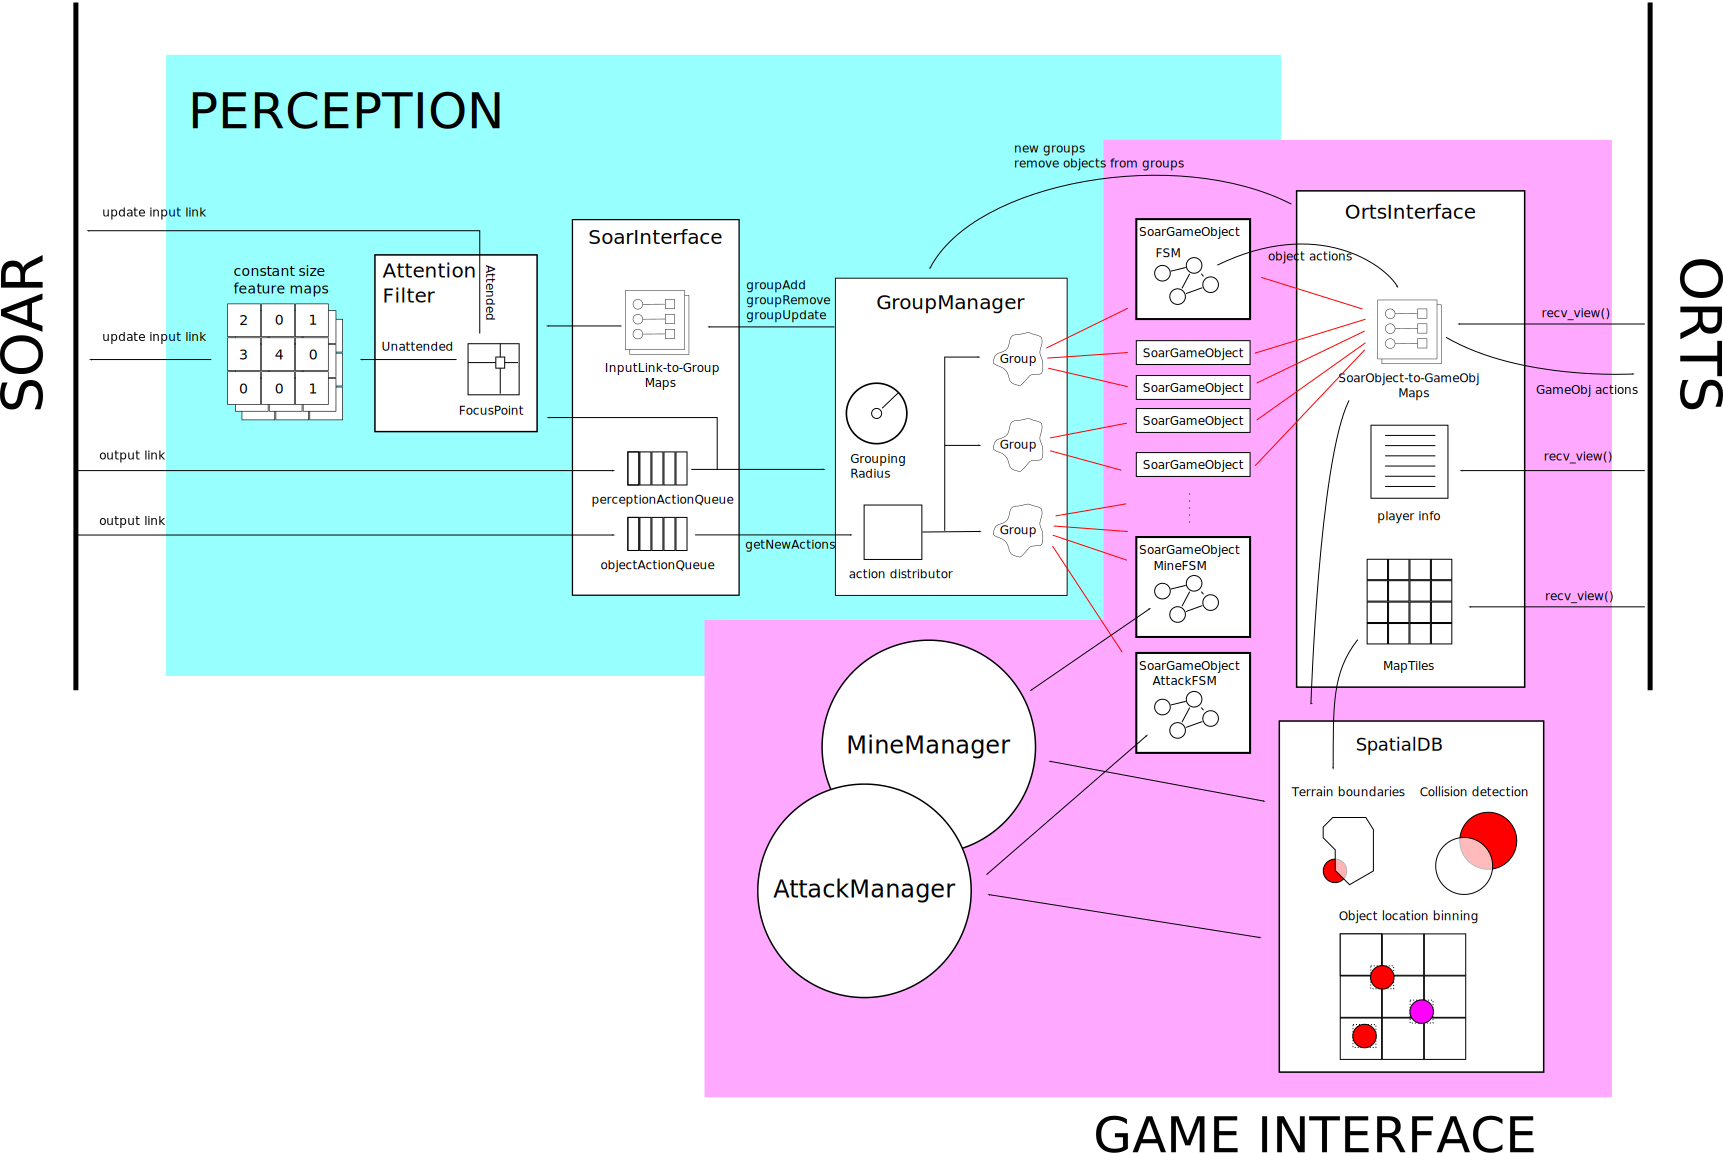
\includegraphics[width=\textwidth]{graphics/middleware_diagram.eps}
\caption{Overview of the modules in Sorts}
\label{fig:SORTSOverview}
\end{figure}

\section{The SORTS Visual System}

During an elaborate RTS game, the amount of information available to the player is massive. Even with a "fog of war" limiting what areas of the map the player has access to, a player can see hundreds (or even thousands) of units, each with its own position, motion, and other attributes. While in general, giving a player more information is a benefit, having no filter on the raw game state would be a hinderance to the player, not only computationally (transferring too many bytes from the middleware to Soar), but also cognitively. Unfiltered information makes abstraction difficult, and makes distinctions involving locality less apparent (for example, seeing that an enemy is within ones base).

A human RTS player has many levels of filtering available, both in the game's GUI interface and the specialized processing of the human visual system. For example, to stage an attack, a player can restrict the GUI's view window to his own base, and see that a group of marines is available. Perhaps one marine needs to be sent as a scout, in that case, the human player can choose to see the marine group as a set of individuals, and choose the best individual to send out. Once the individual has reached its target, the player can again observe (and select) the remaining marines as a group, and send them to attack with one mouse click. This is in contrast to the more complicated unfiltered case, where the player would see the entire map at once, search for marines, reason about whether each individual is close to the base, and perform a separate action to send each to attack.

\subsection{Object Grouping}

The ability of humans to see sets of similar objects as wholes has been well-studied by psychologists. This phenomenon is called Gestalt grouping (\cite{hill99modeling}, \cite{Kubovy1998}). The principles of Gestalt grouping specify that if objects are close together, have common features such as shape, color, and motion, they can be seen as a group. There is some top-down control of this, the observer can choose to see the individuals or the group. We use this concept to give our system the ability to percieve groups of units that are relevant to playing the game. Specifically, we group units by type, owner, and proximity. By default, groups are formed based on all three- groups are formed of units of the same type and owner which are close together. The agent can change the meaning of "close together" by issuing a grouping-radius command to the middleware. Groups are formed by the rule that if a unit of a given class is within the grouping radius of another of the same class, they are in the same group. Note that adjusting this grouping radius to 0 will result in only one unit per group.

The agent also is able to choose to group the objects by owner alone. This is accomplished by issuing an enable-owner-grouping command to the middleware. Grouping by owner allows the agent to view the game at a higher level of abstraction, to see, for example, the locations of the different players' bases and forces.

Actions in the game, such as $attack$ or $move$, are assigned to groups. In the middleware, the execution of each unit is controlled by a separate FSM, so the behavior of the group will not necessarily be uniform. Members of a group can take different paths to a target, and so may become spatially separate as the action is executed. To simplify reasoning in the agent, all groups are automatically set to be "sticky" once an action is assigned to them. In a sticky group, no new members can join, and members are only removed if they are killed. This way, the agent can easily see the results of an action (by checking the status of the group at a later time), and does not get confused when objects executing different actions come close together- all members of a group must be executing the same command. This is analgous to assigning a group a "hotkey" in the user interface of a commercial RTS- the player can quickly get information on a previously-selected group, regardless of what happened to the group since it was last selected. The group will remain sticky until a $free$ command is issued to it, even if all units finish executing the action.


\subsection{Visual Attention}

Even with grouping of objects, the amount of information visible can still be too much. Events in a game such as this tend to occur in restricted spatial areas, and it is worthwhile to present lots of information about a small area, while presenting less information about the rest of the world. 

The human visual system provides some inspiration for a way to do this. A "zoom lens" metaphor is often used to describe human visual attention (\cite{zoomlens}, \cite{hill99modeling}, \cite{anderson})-- some small area of the field of vision is attended to, providing detailed information, while surrounding areas present less and less information. But this area of attention can shift in a guided manner- a human can easily jump to a red object in a sea of black, for example. Feature Integration Theory (FIT) is a common model for describing this kind of "pop-out" effect (\cite{fit}, \cite{anderson}). The basic concept of FIT is that objects not attended to are not present as objects in the visual system, only as features of objects (like colors or shapes). In the red object in a field of black example, the information that something red exists (and its general area) is present whenever the object is in the visual field, but no more information about that object is known until attention selects it. Attention can be directly moved to the red object with no search, but if there were many red objects, any particular one must be found by searching all the red objects, focusing attention on each individually.

These concepts are simple to map onto our system. We simply select a certain number of groups\footnote{Selecting a set number of groups, as opposed to a small region or a number of individuals, not only makes good sense for a video game but is supported by psychological studies \cite{Scholl2001}.} (adjustable by issuing $num-objects$ commands) that are close to a certain point on the map, and provide all information on those groups. Then, for all groups not selected, general information is presented in the form of feature maps. A map for a given feature (enemy units, for example) consists of a list of sectors and associated unit counts. There are 9 sectors, dividing the field of view into a grid. The sectors are numbered with the upper-left as sector0 and the lower right as sector8. For each group that has a given feature, the feature count for the sector the group is centered in is incremented by the number of individuals in the group. Groups that are in attention are not shown in the feature maps.

Using the feature maps, the agent can quickly shift its attentional focus. The commands $look-at-feature$ and $move-to-feature$, which take parameters of a feature name and sector number, cause the focus to jump to the center of one of the groups that shows the chosen feature in the chosen sector. This scheme, in addition to supporting very fast searches, also causes the size of the input link to be constantly bounded, preventing any problems caused by huge amounts of data overwhelming the system.

Beyond grouping and the zoom-lens area of attention, it is possible to restrict the input even further. Capability similar to shrinking a GUI window size (or dealing with a computer screen that can only show so much) is also available- completely cutting out some spatial areas from being percieved. Given our constant-bounded input size, this is no longer needed from a standpoint of avoiding too much data, but can serve to restrict the kind of data available. Specifically, since the feature maps have a set number of sectors, restricting the field of vision serves to increase their resolution. A situation where this is useful is the identification of an enemy unit in an unusual place. If the entire map is always in the field of view, a small area of it being attended to at once, the data in the feature maps will be very low resolution. If the enemy is in many places, it is likely at least one enemy unit will be somewhere in each sector. If one of those sectors also contains a region the agent is trying to control, there is no way of quickly knowing if an enemy is inside or outside the region without attending to it. However, if the agent restricts its field of view to the region in question, an enemy present in the feature map must be an invader, and can quickly be taken care of. An agent that tends to restrict its field of view to its own base while doing tasks there will be able to quickly notice any invaders- they will pop out of its feature maps, regardless of whatever task the agent is attending to.

.. explain commands ..


\section{Low Level Control}

The design philosophy of SORTS requires that Soar agents only issue high
level commands comparable to those that would be expected from a human
player. The reason human players of commercial RTS games do not have to
worry (too much) about micromanagement is because much of it is handled
for them by the game engine. Likewise, in SORTS, we handle low-level
micromanagement with our middleware so that Soar does not have to. This
is achieved by assigning each controllable unit a behavior specified
as an finite state machine. Soar only has to specify which behavior a
unit should take on, and the FSM will control the unit in predictable
ways. We have already programmed a basic library of behaviors, listed in
figure~\ref{fig:implementedBehaviors}.

\subsection{Behaviors as Finite State Machines}

The main functionality of a behavior resides in its {\tt update}
function. This function is called for all living, controllable units
whenever the higher level function \verb|updateGroups()| is called in
the ORTS event handler (see section~\ref{sec:OrtsEventHandler}). This
means that the {\tt update} function for every active behavior is called
once everytime SORTS receives a viewframe from the ORTS server, which is
the smallest unit of discernable state change.

During the {\tt update} call, the behavior decides which low-level action
provided by the ORTS API, or lack thereof, to execute for the game
object which it controls. This decision is made based on the behavior's
current state and also the state of the game object, which it as direct
access to, unlike the Soar agent. The behavior also decides which state
to transition to for the next {\tt update} call.

\subsubsection{Coordination Managers}

During preparations for the first ORTS tournament, it was decided that
certain behaviors that required high levels of coordination amongst
each other needed to have access to more information than just game
object state if they were to perform well enough to be competitive in
the tournament. Therefore, two behaviors, one that controls mining and
one that controls attacking, were written to have access to a bigger
picture of the overall game state via communication with coordinating
mechanisms called we called "managers."

The result was that the behaviors themselves were relatively simple.
During every {\tt update} call, a managed behavior just asks the manager
it was assigned to what it should do, and then does it. The advantage to
using such an approach is that the manager can keep track of what each
behavior it controls is doing, and coordinate sophisticated strategies
such as optimal assignment of miners to mineral patches, or focusing the
firepower of many units on one enemy at a time.

\subsubsection{Default Behaviors}

There are some actions that are always advantageous to do. For example,
if an offensive unit passes within firing range of an enemy unit, it is
almost always better to attack the enemy unit given that there is not a
more important target to attack. We don't want to burden a Soar agent
with having to detect every opportunity to perform such actions, so
game units can be assigned default behaviors. The desired behavior in
the situation described above is implemented by the {\tt AttackNearFSM}
default behavior, which fires on nearby targets whenever they are in
range and the controlled unit was not explicitly ordered to fire on
something else.

As opposed to assigned behaviors, default behaviors are specified
when units are created rather than when they are first desired, and
a single in-game unit can have several default behaviors at once.
It is important that a default behavior not override the actions
of an assigned behavior. For example, the default behavior for a
unit to run away when being attacked should not be manifested if the
unit was assigned the move behavior in the opposite direction of the
retreat. However, there is no built-in mechanism to ensure this kind of
suppression in SORTS yet, so it is the responsibility of the default
behavior to make sure it doesn't obstruct assigned behaviors.

\begin{figure}
\begin{center}
\begin{minipage}{5in}
\begin{tabular}{|l|p{1.0in}|p{3.0in}|}
\hline
Behavior name     & Parameters     & Description\\ 
\hline\hline
AttackFSM         & id             & Attack group with specified id \\ 
\hline
AttackNearFSM     &                & Attack any enemy target within range,
                                     except when already attacking another
                                     target                         \\
\hline
BuildFSM          & t, x, y        & Build a building of type t at (x, y) \\ 
\hline
MineFSM           &                & Mine for minerals              \\
\hline
MoveFSM           & x, y, speed    & Object tries to pathfind and move
                                     to coordinate (x, y)           \\
\hline
TrainFSM          & t              & Train a unit of type t         \\
\hline

\end{tabular}
\end{minipage}
\end{center}
\caption{A list of implemented behaviors.}
\label{fig:implementedBehaviors}
\end{figure}


\section{Updating the Game State}

\subsection{Raw State Information}

The ORTS API provides complete game state update information in the form
of 6 lists:

\begin{itemize}
  \item \verb|new_tile_indexes| New game tiles encountered via
  uncovering of fog of war.
  \item \verb|new_objs| New game objects, such as enemy units and
  buildings, or world objects such as trees.
  \item \verb|changed_objs| Game objects that have changed since the
  previous viewframe.
  \item \verb|vanished_objs| Game objects that disappeared from the
  player's vision.
  \item \verb|dead_objs| Game objects that died.
  \item \verb|new_boundaries| New terrain boundaries that demarcate
  the border between different terrain types, such as ground and cliff.
\end{itemize}

SORTS currently takes into account the information in all
the lists except \verb|new_tile_indexes| and
\verb|new_boundaries|. The former is ignored because SORTS
currently does not have any functioning capability to reason about
terrain, except for collision detection. The latter is ignored because
we get this information from the game tiles directly whenever we check
for boundaries. Note also that currently, SORTS treats objects vanishing
(reported in \verb|vanished_objs|) and objects dying (reported in
\verb|dead_objs|) as one and the same thing. This will probably change
in the future as agents use more sophisticated reasoning.

All game state updates, both internal to the middleware and to the Soar
input link, are performed in the ORTS event handler, which is triggered
everytime the middleware receives a new viewframe from the ORTS server.
An overview of the flow of control among the various functions is shown
in figure~\ref{fig:flow}. Detailed descriptions of the two event
handlers are provided below.

\begin{figure}
\includegraphics[width=\textwidth]{graphics/flow.eps}
\caption{Overview of how control is passed through Sorts. Note that the
two gray regions represent two different threads executing
asynchronously.}
\label{fig:flow}
\end{figure}

\subsection{The ORTS Event Handler}
\label{sec:OrtsEventHandler}

The ORTS event handler is triggered everytime the middleware receives
a new viewframe from the ORTS server. This event handler and the
Soar event handler are the main functions from which most other
function calls are made. Pseudo-code for the handler is shown in
figure~\ref{fig:OrtsEventHandler}.

\begin{figure}
\begin{verbatim}
ORTSEventHandler
  lockMutex()
  mergeChanges(oldChanges, changes)
  if currentViewFrame - lastActionFrame > ALLOWED_LAG then
    unlockMutex()
    return
  end
  removeDeadObjects(changes)
  assignSoarActions()
  updateSoarGameObjects(changes)
  sendActions()
  updateGroups()
  unlockMutex()
end
\end{verbatim}
\caption{Pseudo code for the ORTS event handler}
\label{fig:OrtsEventHandler}
\end{figure}

Each function call is described below.

\begin{itemize}

\item \verb|lockMutex()| and \verb|unlockMutex()|
  This mutex locks the Soar event handler from executing until the
  ORTS event handler is finished. This is important since we don't want
  the Soar command buffer to change while we are processing that buffer.

\item \verb|mergeChanges(oldChanges, changes)|
  If SORTS falls behind the ORTS server too much, changes to the game
  state will be accumulated but not processed in the interest of
  catching up. This function merges changes reported in previous
  viewframes with the current changes.

\item \verb|removeDeadObjects(changes)|
  This function removes all game objects that have just died or vanished
  in the current frame. This call needs to be made before the call to
  \verb|assignSoarActions()| so that we don't try to assign any actions
  to objects that disappeared, which the ORTS server would not
  understand.

\item \verb|assignSoarActions()|
  Interprets commands queued from the Soar output-link as ORTS actions and
  distributes them to the appropriate groups. The actions are not sent
  to the ORTS server until \verb|sendActions()| is called.

\item \verb|updateSoarGameObjects(changes)|
  This is the main function that updates the attributes of the
  SoarGameObject structures in the middleware. It is called after
  \verb|assignSoarActions()| so that units will begin responding to
  their commands in the Soar cycle that immediately follows the one in
  which they were assigned.

\item \verb|sendActions()|
  This is a call to the ORTS API that sends all queued actions to the
  server.

\item \verb|updateGroups()|
  Runs the grouping algorithm over SoarGameObjects that have changed or
  appeared, and prunes those groups whose members have died. These
  changes are directly reflected in the Soar input-link, but are
  buffered in the SML interface until the next Soar decision cycle.

\end{itemize}

\subsection{The Soar Event Handler}
\label{sec:SoarEventHandler}

The Soar event handler is triggered at the end of each Soar decision
cycle. The main responsibility of this function is to take commands off
the Soar output-link and buffer them into action queues in the
middleware.

\begin{figure}
\begin{verbatim}
SoarEventHandler
  lockMutex()
  if Catchup = true then
    unlockMutex()
    return
  end if
  getNewSoarOutput()
  processVisionCommands()
  processGameCommands()
  unlockMutex()
end
\end{verbatim}
\caption{Pseudo code for the Soar event handler}
\label{fig:SoarEventHandler}
\end{figure}

Figure~\ref{fig:SoarEventHandler} shows the pseudo-code for the
function. The following is a list of descriptions for each call made in
the function.

\begin{itemize}

\item \verb|lockMutex()| and \verb|unlockMutex()|
  These calls lock on the same mutex as the ORTS event handler, thereby
  making the execution of these two functions mutually exclusive.

\item \verb|getNewSoarOutput()|
  Takes all commands on the Soar output-link and queues them into lists
  in the middleware. This includes both commands issued to in-game units
  as well as commands that adjust middleware parameters such as grouping
  radius and center of visual attention. However, none of the commands
  are actually processed by this function.

\item \verb|processVisionCommands()|
  Processes Soar commands related to the perceptual system. These
  commands include changing the grouping radius, looking at a specific
  coordinate, looking at a feature in the feature map, and changing the
  maximum number of objects allowed on the input-link at any time (for
  a complete list, see section~\ref{sec:output-link}. These commands
  are processed here rather than with the in-game commands because Soar decision cycles can occur much faster than ORTS events.

\item \verb|processGameCommands()|
  Handles all commands that affect the way the middleware executes
  low-level actions, such as in the FSMs, but do not translate directly
  into ORTS game object actions. Also handles miscellaneous queries that
  Soar may make to the middleware for information not normally provided
  to it. Currently, there are only three such commands: finding a
  location for a building, and setting and clearing the mineral buffer
  (see section~\ref{sec:output-link}).

\end{itemize}


\section{Soar IO Description}

\subsection{The SORTS input-link}

There are five top-level attributes on the SORTS input link, "groups", "game-info", "feature-maps", "vision-info", and "query-results". The groups, feature-maps, and vision-info structures are all part of the main visual system (see XXX), while game-info contains higher-level information about the game world, and query-results is used to communicate the results of specialized queries from Soar to the middleware.

The exact data structures are as follows:

\begin{center}
\begin{tabular}{|l|p{4.0in}|}
\hline
\multicolumn{2}{|c|}{\textbf{Attributes of io.input-link}}\\ 
\hline
attribute  &  description\\
\hline \hline
\multicolumn{2}{|l|}{\textbf{vision-info structure:}}\\ 
\hline
vision-info & Contains information on the current state of the vision system. \\
\hline
vision-info.center-x & The coordinate of the center of the region in view. \\
vision-info.center-y & \\
\hline
vision-info.focus-x & The coordinate of the center of focus (spotlight of attention). \\
vision-info.focus-y & \\
\hline
vision-info.num-objects-visible & The maximum number of objects (groups) present on the input-link. All other objects within the view window are present in feature maps. \\
\hline
vision-info.grouping-radius & All objects of the same type (except as below) and owner within this distance of each other are in the same group (set to 0 for individuals). \\
\hline
vision-info.owner-grouping & Ignore type when grouping, only group by owner (1 if enabled, 0 if disabled). \\
\hline
\multicolumn{2}{|l|}{\textbf{groups structure:}}\\ 
\hline
groups & The set of groups being attended to. \\
\hline
groups.group & Multi-valued, one instance for each group. Detailed below. \\
\hline
\multicolumn{2}{|l|}{\textbf{feature-maps structure:}}\\ 
\hline
feature-maps & Contains all feature maps- low-resolution information about certain features of unattended (but visible) objects. \\
\hline
feature-maps.friendly & Friendly feature map- each friendly unit (not group) results in one instance of this feature, marked in the sector of the group's center of gravity. \\
\hline
feature-maps.friendly-workers & A subset of the friendly feature map, showing only workers.\\
\hline
feature-maps.enemy & Similar to the above, but for enemy units.\\
\hline
feature-maps.minerals & Similar to the above, but for minerals.\\
\hline
feature-maps.moving-units & Moving units (if grouping is used, one moving object causes the whole group to be seen as moving).\\
\hline
feature-maps.(any).sector0 & Feature counts for each of the nine sectors. 0 is the upper left, 8 is the lower right.\\
.. & \\
feature-maps.(any).sector8 & \\
\hline
\multicolumn{2}{|l|}{\textbf{game-info structure:}}\\ 
\hline
game-info & General information about the game (non-visual information).\\
\hline
game-info.num-players & The number of players.\\
\hline
game-info.player-id & The ID number of the Soar player.\\
\hline
game-info.map-xdim & The dimensions of the game map. \\
game-info.map-ydim & \\
\hline
game-info.view-frame & The last view frame handled by the middleware (the number of game cycles executed).\\
\hline
game-info.my-minerals & Minerals available to the player. \\
\hline
game-info.mineral-buffer & The number of minerals to reserve for certain tasks (see section XXX).\\
\hline
game-info.worker-count & The number of units of each type owned by the player. \\
game-info.marine-count & \\
game-info.tank-count & \\
\hline
\multicolumn{2}{|l|}{\textbf{query-results structure:}}\\ 
\hline
query-results & The result of the last query to the middleware.\\
\hline
query-results.query-name & The name of the last query executed.\\
\hline
query-results.param0 & Query return values- the meaning of these is dependant on the query-name. \\
query-resutls.param1 & \\
\hline

\end{tabular}

\begin{tabular}{|l|l|p{3.5in}|}
\hline
\multicolumn{3}{|c|}{\textbf{Attributes of io.input-link.groups.group objects}}\\ 
\hline
attribute  & which groups &  description\\
\hline \hline
num-members & all & The number of individuals comprising the group. \\
\hline
type & all &The type of the group (ex: worker, mineral). \\
\hline
x-pos & all &The x,y location of the center of gravity of the group.\\
y-pos & & \\
\hline
x-min & all &The bounding box of the group.\\
x-max & & \\
y-min & & \\
y-max & & \\
\hline
health & all &The sum of the health of all units in the group.\\
\hline
taking-damage & all &The number of members of the group currently taking damage (under attack). \\
\hline
shooting & all &The number of members of the group currently attacking an enemy. \\
\hline
speed & all &The average speed of the group. \\
\hline
heading & all &The average heading of the group. \\
\hline
dist-to-focus & all &The distance from the center of gravity of the group to the attentional focus point.\\
\hline
dist-to-query & all &The distance from the center of gravity of the group to the last query location.\\
\hline
owner & all &The player number of the group's owner.\\
\hline
enemy & all &1 if the group belongs to an enemy player, 0 otherwise.\\
\hline
sticky & friendly & 1 if the group is sticky- sticky groups remain together even if they are no longer spatially close.\\
\hline
command & friendly & The last command issued to the group ("none" if no command has been issued).\\
\hline
command-running & friendly & The number of members of the group currently executing a command.\\
\hline
command-success & friendly & The number of members of the group that successfully completed the last command.\\
\hline
command-failure & friendly & The number of members of the group that unsuccessfully completed the last command.\\
\hline
minerals & friendly workers & The total number of minerals possessed by the workers in the group.\\
\hline
active-mining & friendly workers & The number of workers that are actively mining.\\
\hline
\end{tabular}
\end{center}

\subsection{The SORTS output-link}

The output-link allows the Soar agent to act in the game world by issuing commands to groups of friendly units, communicate directly to the middleware for actions such as querying,
and adjust the parameters of the visual subsystem in the middleware. All structures on the output link are similar- the Soar agent creates an output-link.command object with a name (\textbf{output-link.command.name}) specified. Depending on the command name, different parameters are needed. Parameters are attached to the command structure, as in \textbf{output-link.command.param0}. All legal commands and their necessary parameters are detailed below.


\begin{center}
\begin{minipage}{6.5in}
\begin{tabular}{|l|p{1.0in}|p{3.5in}|}
\hline
\multicolumn{3}{|c|}{\textbf{Soar output-link commands}}\\ 
\hline
command name &  parameters & description \\
\hline \hline
\multicolumn{3}{|l|}{\textbf{Vision commands}}\\ 
\hline
grouping-radius & $value$ & Change the grouping radius of the vision system. \\
\hline
enable-owner-grouping & (none) & Enable grouping-by-owner.\\
\hline
disable-owner-grouping & (none) & Disable grouping-by-owner.\\
\hline
change-view-width & $value$ & Change the width of the agent's view to be $value$.\\
\hline 
look-at-location & $x,y$ & Move the focus of attention to the given coordinate (which must be in the current view window.\\
\hline
move-to-location & $x,y$ & Shift the view window to be centered at the given coordinate, and make that the focus of attention. \\
\hline
look-at-feature & $feature$, $sector$ & Move the focus of attention to a given feature in a given sector. The legal features are the names of the feature-map objects on the input link.\\
\hline
move-to-feature & $feature$, $sector$ & As above, but re-center the view window to the new location, also.\\
\hline
num-objects & $value$ & Change the maximum number of objects (groups) present on the input-link at once.\\
\hline
\multicolumn{3}{|l|}{\textbf{General middleware commands}}\\ 
\hline
locate-building & $building$, $x,y$, $distance$ & This command requests that the middleware attempt to find a location for a building of type $building$ approximately $distance$ units from the coordinate given. The resulting coordinate is returned through the query-result structure on the input-link. \\
\hline
increase-mineral-buffer & $value$ & Increase the mineral buffer by $value$ minerals.\\
\hline
clear-mineral-buffer & (none) & Set the mineral buffer to 0.\\
\hline
\multicolumn{3}{|l|}{\textbf{Group commands}}\\
\hline
move & $group0$, $param0$, $param1$ & Move the group with ID $group0$ to the x,y location where $param0$ is x and $param1$ is y, using the default precision of 10 (allow units to complete successfully if they are within 10 of the target).\\
\hline
move & $group0$, $param0$, $param1$, $param2$ & Move group $group0$ to the x,y location where $param0$ is x and $param1$ is y, using a precision of $param2$.\\
\hline
build & $group0$, $param0 .. param3$ & Use group $group0$ to build a building of type $param0$\footnote{Legal building types: 0=controlCenter, 1=barracks, 2=factory} at the x,y location given by $param1, param2$. If $param3$ is 1, the mineral buffer is used, otherwise it is not. \\
\hline
train & $group0$, $param0 .. param2$ & Use group $group0$ (a building) to train units of type $param1$\footnote{Legal unit types: 0=worker, 1=marine, 2=tank}. Train up to $param2$ units, and use the mineral buffer if $param3$ is 1. \\
\hline
attack & $group0$, $group1$ & Use the friendly group with ID $group0$ to attack $group1$.\\
\hline
mine & $group0$ & Assign $group0$ to mine minerals. The control center and mineral patch to use are automatically determined in the middleware. \\
\hline
stick & $group0$ & Set $group0$'s to be sticky- ensure it stays as one group, even if the members move apart. Assigning any of the above actions to a group does this by default. \\
\hline
free & $group0$ & Clear $group0$'s sticky status- allow the members to be split up and join other groups.\\
\hline
join &  $group0$, $group1$ & Force $group0$'s members to join $group1$. If $group1$ is not sticky, this may be automatically undone the next cycle.\\
\hline
\end{tabular}
\end{minipage}
\end{center}


\bibliographystyle{plain}
\bibliography{report}

\end{document}
